\chapter{Branch Coverage}

\section{Introduction}
This chapter details my effort to implement branch coverage. The structure of the chapter is largely the same as the previous chapter. However, there is a lot more detail provided on the algorithm as it is thought to be the only detailed description on the process of converting an Abstract Syntax Tree to a Control Flow Graph.

\section{Analysis}

As detailed in the literature review, branch coverage is how many conditional statements have had all possible paths executed. So for an \verb|if| statement, if it only ever evaluates to \verb|true| then the branch coverage at that vertex is 50\%. This becomes a problem when you have code such as in Figure \ref{lst:branchingExample}.If the \verb|if| statement always evaluates to true during testing, statement coverage will show as being over 99\%. However, if it ever evaluates to false then \verb|someObject| won't be initialised, and an exception will be thrown later on if somewhere else \verb|someObject| is referenced.

\begin{figure}
\centering
\begin{minipage}{.33\textwidth}
  \centering
  \lstinputlisting{code/branch_example.java}
  %\caption{Some sample pseudocode}
  \label{lst:branchingExample}
\end{minipage}%
\begin{minipage}{.5\textwidth}
  \centering
  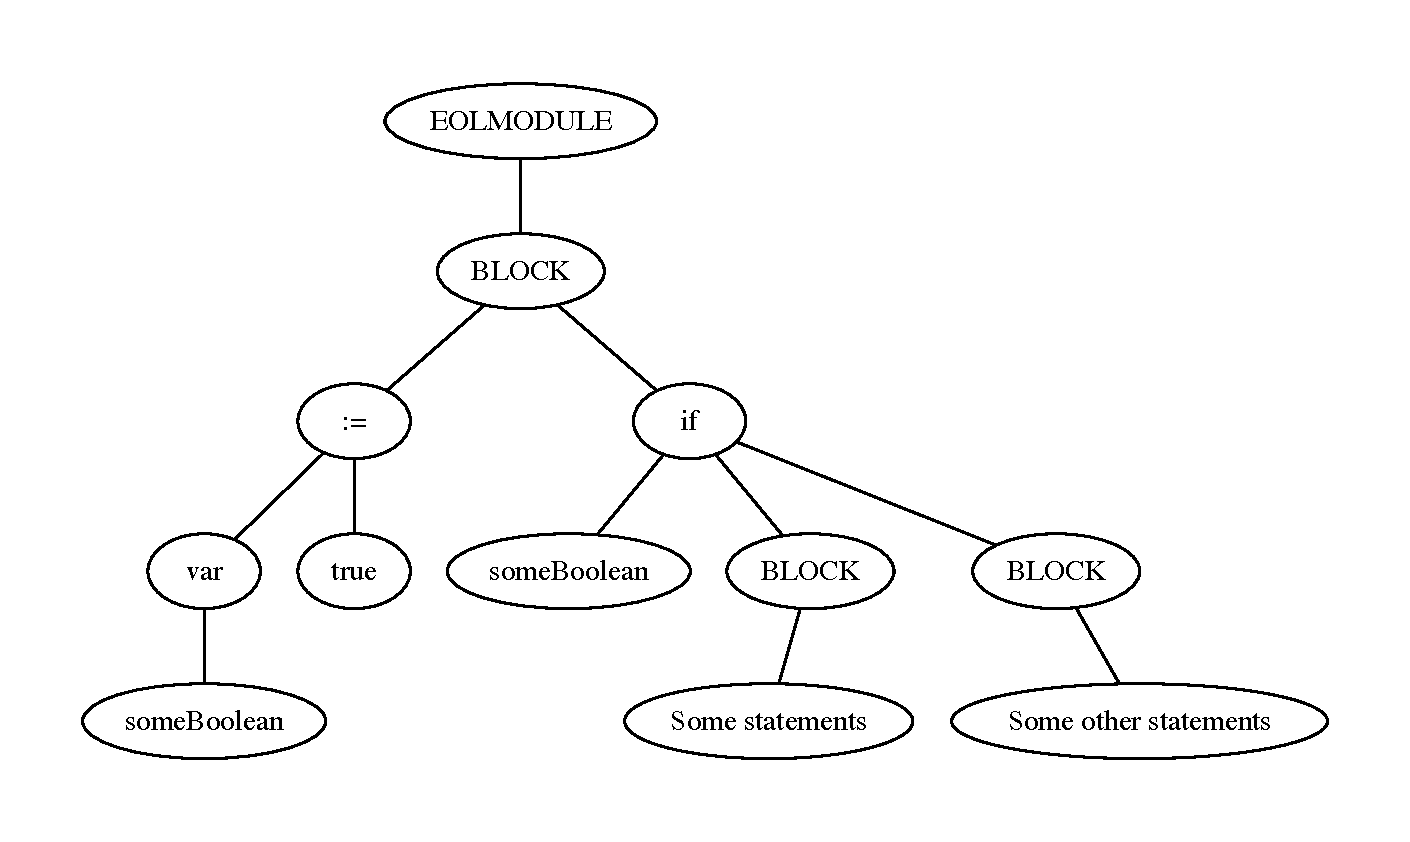
\includegraphics[scale=0.5]{figures/branchSampleAST.pdf}
  %\caption{The AST of the program in Figure \ref{lst:branchingExample}}
  \label{fig:branchExampleAST}
\end{minipage}
\caption{On the left is some sample pseudocode, and on the right is the AST for the sample pseudocode}
\end{figure}

Branch coverage can counter this by looking at how many of the possible paths after all conditional statements have been executed. So in the code in Figure \ref{lst:branchingExample}, only 50\% of possible paths from that \verb|if| statement have been executed, and so the branch coverage is 50\%.

By looking at the AST (Figure \ref{fig:branchExampleAST}) of the sample code, it would appear that by counting the number of blocks below the \verb|if| vertex, we could determine how many branches in the code there are, and after execution we could see how many of those branches have been executed.

Unfortunately this approach is not perfect. The blocks only appear when curly braces are used. If just a single statement is placed under the \verb|if| statement, then the block is skipped and just a vertex for the single statement appears. So this means that the code is now more complex than it was previously thought to be. Furthermore, \verb|if| statements can have children that never need to be executed (because they just contain information about the conditional), and so my algorithm would need to include details of this. If these were the only drawbacks then I would still choose this approach. However, this kind of caveat occurs for many conditional statements, and so the code that would be produced would be rather unwieldy and difficult to maintain.

The approach therefore that I have chosen to take is actually quite difficult to justify. I suggest that the AST be converted to a Control Flow Graph (CFG), at which point the branches from each vertex will be clear. A record will be made on which edges between vertices have been executed, and the total number of edges will be counted. The edges that have not been recorded will map to the branches that were not taken. The reason that this is difficult to justify is that an extensive search has not come up with any explicit instructions on how to go about generating a control flow graph from an abstract syntax tree. Furthermore, the complexities of special code for each type of statement will still apply when performing the conversion. However, some forward thinking means that the conversion from AST to CFG will be necessary when performing the path coverage because of the formula detailed in the literature review's path coverage section to calculate cyclomatic complexity, and so this effort will solve two problems, and will have a quicker overall development time.

Before beginning development, a list was made of the statements that need to be included. This was done by going through the Epsilon book \citep{epsilonBook} which is a complete source of EOL syntax, but also as well by going through the EuGENia source to see which statements are actually used in real EOL code. The list was then loosely ordered in priority based on the number of uses within the EuGENia source. The list as as follows:

\begin{enumerate}[nolistsep]
\item block
\item if
\item if .. else
\item for
\item while
\item switch
\item case
\item default
\item operation
\item return
\item break
\item breakAll
\end{enumerate}

For each of the identified statements, I will individually analyse how they can be converted from an AST to a CFG. For each statement a sample AST will be shown, as well as the desired CFG.

\subsection{The Block}
Block is not actually a statement, but refers to a block of statements. Within a block can be any other set of statements, including other blocks. The contents of a block are often contained within \{ \} braces, but not always (see the case statement).

The block is not conditional in any way. It can have a number of children, which are executed in order of first child (left-most) to last child (right-most). During the conversion of AST to CFG, when a block is encountered it should simply be a case of joining a block vertex from the last statement that was encountered, and joining it to the the block's first child.

The code in Figure \ref{fig:block} is a whole EOL program. The whole program is inside a block statement, as can be seen by the AST in the same figure. There are two statements in the block, and in the AST each statement is represented as a child. In the CFG, each of the children are represented sequentially, so the first child is represented after the block, and then the second child after the first child.

The block could be left out of the CFG, as arguably it does not provide any more information about control flow. For the time being this will be ignored, but at a later stage I will discuss and decide on this. For the rest of this analysis, the block statement may be used to represent any subset of vertices that does not add to the analysis. The input to the block vertex will represent input to the first vertex of the subset, and the output from the block will represent the output from any possible exit vertices from the subset.

\begin{figure}
\centering
\begin{minipage}{.3\textwidth}
  \centering
  \lstinputlisting{code/statements/block.java}
  %\caption{}
  %\label{lst:blockStatement}
\end{minipage}%
\begin{minipage}{.3\textwidth}
  \centering
  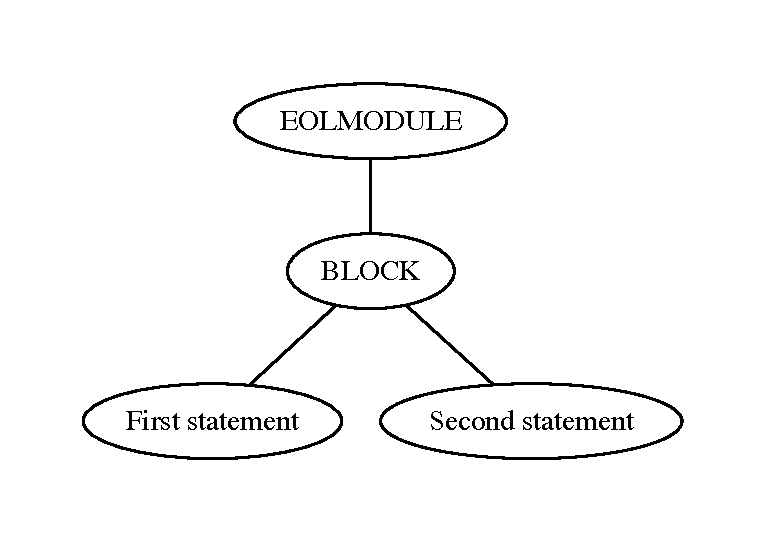
\includegraphics[width=\linewidth]{figures/statements/block_AST.pdf}
   % \caption{}
  %\label{fig:blockAST}
\end{minipage}
\begin{minipage}{.3\textwidth}
  \centering
  \includedot[scale=0.5]{figures/statements/block_CFG}
   % \caption{}
  %\label{fig:blockCFG}
\end{minipage}
\caption{From left to right: The block's code, AST and desired CFG}
\label{fig:block}
\end{figure}

\subsection{The if statement}

The if statement is going to be treated as a separate statement to the if .. else statement, because when it comes to designing and implementing the algorithm, different code will be required for each.

The if statement evaluates its parameter, and if it evaluates to true then it executes the code in the parenthesis that follow it, or if there are no parenthesis, it executes the statement that directly follows it. While the outcome of execution is the same (when there is only one statement executed following an if statement that evaluates to true), the use of parenthesis following the if statement changes the structure of the AST in a way that must be considered during the conversion. Figure \ref{fig:if} shows the if statement that uses parenthesis, and figure \ref{fig:ifnoparen} shows the statement that does not use parenthesis.

When the parenthesis are used, if the if statement evaluates to false then the statement that immediately follows the block must be the next statement to be executed. This will be the sibling of the if statement in the AST. If the if statement evaluates to true, then once it has finished executing the block it must move on to the next statement after the block, which again will be the next sibling of the if statement in the AST.

When no parenthesis are used, the same rules almost apply. Except that rather than looking for the next statement after the block, it will be the second statement following the if statement. This will still be represented in the AST as the next sibling of the if statement.
\begin{figure}
\centering
\begin{minipage}{.3\textwidth}
  \centering
  \lstinputlisting{code/statements/if.java}
  %\caption{}
  %\label{lst:blockStatement}
\end{minipage}%
\begin{minipage}{.3\textwidth}
  \centering
  \includedot[width=\linewidth]{figures/statements/if_AST}
   % \caption{}
  %\label{fig:blockAST}
\end{minipage}
\begin{minipage}{.3\textwidth}
  \centering
  \includedot[scale=0.5]{figures/statements/if_CFG}
   % \caption{}
  %\label{fig:blockCFG}
\end{minipage}
\caption{From left to right: The if statement with parenthesis' code, AST and desired CFG}
\label{fig:if}
\end{figure}

\begin{figure}
\centering
\begin{minipage}{.3\textwidth}
  \centering
  \lstinputlisting{code/statements/ifnoparen.java}
  %\caption{}
  %\label{lst:blockStatement}
\end{minipage}%
\begin{minipage}{.3\textwidth}
  \centering
  \includedot[width=\linewidth]{figures/statements/ifnoparen_AST}
   % \caption{}
  %\label{fig:blockAST}
\end{minipage}
\begin{minipage}{.3\textwidth}
  \centering
  \includedot[scale=0.5]{figures/statements/ifnoparen_CFG}
   % \caption{}
  %\label{fig:blockCFG}
\end{minipage}
\caption{From left to right: The if statement without parenthesis' code, AST and desired CFG}
\label{fig:ifnoparen}
\end{figure}

\subsection{The if .. else statement}

The if .. else statement differs from the if statement in two ways. The first is that control flow will always go down one of two paths, rather than potentially going down one or skipping around it. Secondly, the if statement in the AST now has three children rather than just two. The additional child is the block (or single statement if no parenthesis are used) for the else statement.

When implementing the conversion a check will need to be implemented to see how many children the if statement has. While the EOL language defines an else statement, it is never featured in the AST that is generated and therefore cannot be used to distinguish between an if statement and an if .. else statement.

\begin{figure}
\centering
\begin{minipage}{.3\textwidth}
  \centering
  \lstinputlisting{code/statements/ifelse.java}
  %\caption{}
  %\label{lst:blockStatement}
\end{minipage}%
\begin{minipage}{.3\textwidth}
  \centering
  \includedot[width=\linewidth]{figures/statements/ifelse_AST}
   % \caption{}
  %\label{fig:blockAST}
\end{minipage}
\begin{minipage}{.3\textwidth}
  \centering
  \includedot[scale=0.5]{figures/statements/ifelse_CFG}
   % \caption{}
  %\label{fig:blockCFG}
\end{minipage}
\caption{From left to right: The if .. else statement without parenthesis' code, AST and desired CFG}
\label{fig:ifelse}
\end{figure}

\subsection{The while loop}

\begin{figure}
\centering
\begin{minipage}{.3\textwidth}
  \centering
  \lstinputlisting{code/statements/while.java}
  \caption{}
  \label{lst:whileBranch}
\end{minipage}%
\begin{minipage}{.3\textwidth}
  \centering
  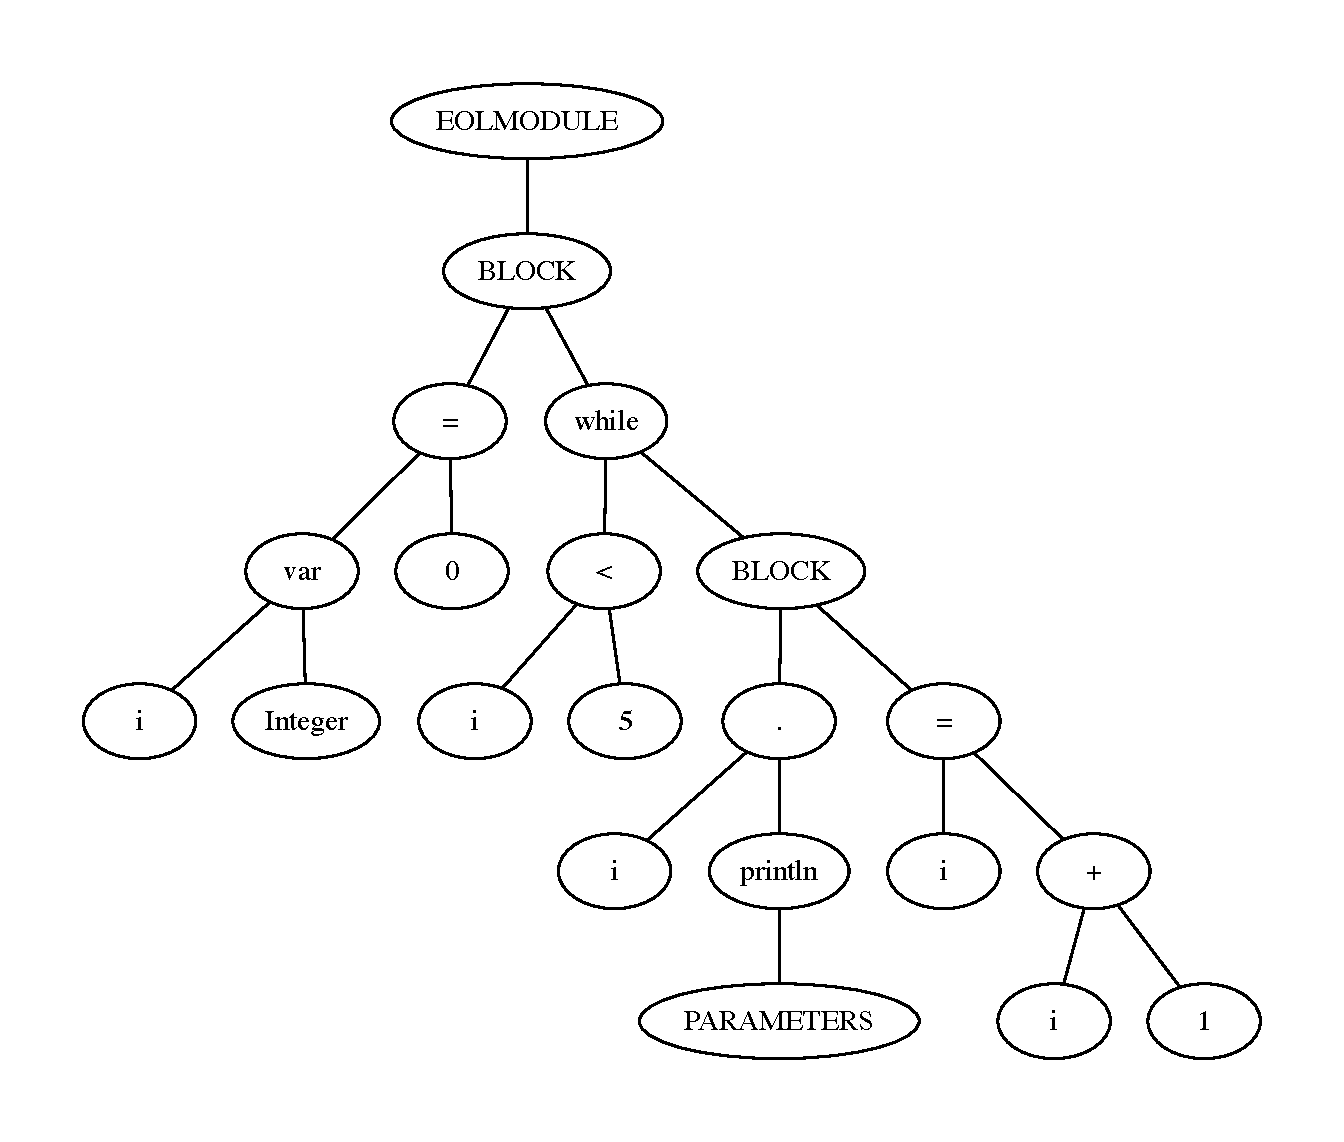
\includegraphics[width=\linewidth]{figures/statements/while_AST.pdf}
    \caption{}
  \label{fig:whileAST}
\end{minipage}
\begin{minipage}{.3\textwidth}
  \centering
  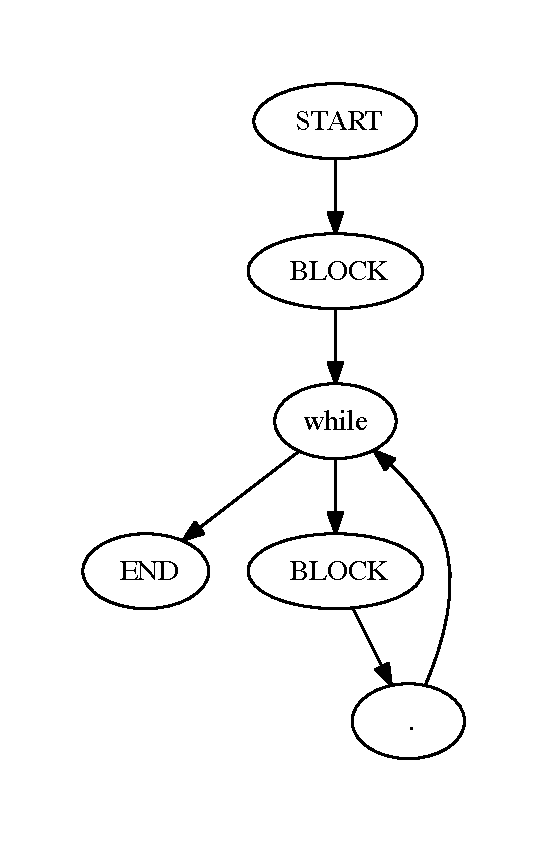
\includegraphics[scale=0.5]{figures/statements/while_CFG.pdf}
    \caption{}
  \label{fig:whileCFG}
\end{minipage}
\end{figure}